% ETH Zurich  - 3D Photography 2015
% http://www.cvg.ethz.ch/teaching/3dphoto/
% Template for project proposals

\documentclass[11pt,a4paper,oneside,onecolumn]{IEEEtran}

\usepackage{graphicx}
\usepackage[square,numbers]{natbib}
\usepackage{url}
\usepackage{hyperref}
\usepackage[nameinlink]{cleveref}
\usepackage{subcaption}
\usepackage[inline]{enumitem}
%\usepackage[autostyle]{csquotes}

% Enter the project title and your project supervisor here
\newcommand{\ProjectTitle}{Semantic Feature Localization}
\newcommand{\ProjectSupervisor}{Marcel Geppert}
\newcommand{\DateOfReport}{March 13, 2020}

% Enter the team members' names and path to their photos. Comment / uncomment related definitions if the number of members are different than 2.
% Including photographs are optional. Photos are there to help us to evaluate your group more effectively. If you wish not to include your photos, please comment the following line.
%\newcommand{\PutPhotos}{}
% Please include a clear photo of each member. (use pdf or png files for Latex to embed them in the document well)
\newcommand{\memberone}{Pedro Aparicio}
\newcommand{\memberonepicture}{pic1.png}
\newcommand{\membertwo}{Christian Leopoldseder}
\newcommand{\membertwopicture}{pic1.png}
\newcommand{\memberthree}{Sahan Paliskara}
\newcommand{\memberthreepicture}{pic2.png}
\newcommand{\memberfour}{Patricia Sung}
\newcommand{\memberfourpicture}{pic1.png}

%%%% DO NOT EDIT THE PART BELOW %%%%
\title{\ProjectTitle}
\author{3D Vision Project Proposal\\Supervised by: \ProjectSupervisor\\ \DateOfReport}
\begin{document}
\maketitle
\vspace{-1.5cm}\section*{Group Members}\vspace{0.3cm}
\begin{center}\begin{minipage}{\linewidth}\begin{center}
\begin{minipage}{3 cm}\begin{center}\memberone\ifdefined\PutPhotos\\\vspace{0.2cm}\includegraphics[height=3cm]{\memberonepicture}\fi\end{center}\end{minipage}
\ifdefined\membertwo\begin{minipage}{3 cm}\begin{center}\membertwo\ifdefined\PutPhotos\\\vspace{0.2cm}\includegraphics[height=3cm]{\membertwopicture}\fi\end{center}\end{minipage}\fi
\ifdefined\memberthree\begin{minipage}{3 cm}\begin{center}\memberthree\ifdefined\PutPhotos\\\vspace{0.2cm}\includegraphics[height=3cm]{\memberthreepicture}\fi\end{center}\end{minipage}\fi
\ifdefined\memberfour\begin{minipage}{3 cm}\begin{center}\memberfour\ifdefined\PutPhotos\\\vspace{0.2cm}\includegraphics[height=3cm]{\memberfourpicture}\fi\end{center}\end{minipage}\fi
\ifdefined\memberfive\begin{minipage}{3 cm}\begin{center}\memberfive\ifdefined\PutPhotos\\\vspace{0.2cm}\includegraphics[height=3cm]{\memberfivepicture}\fi\end{center}\end{minipage}\fi
\end{center}\end{minipage}\end{center}\vspace{0.3cm}
%%%% END OF PROTECTED LINES %%%%


%%%% BEGIN WRITING THE DOCUMENT HERE %%%%


%Document name: 3DVision_Proposal_Aparicio_Leopoldseder_Paliskara_Sung.pdf

\section{Description of the project}
% A high level description of the project, mentioning the main goal, the input and planned output data. Typically 4-5 sentences, also citing immediately related literature \cite{paper}.

A possible approach for an autonomous car to localize itself is using a pre-computed map as a prior.
This map can be queried to compute a location estimate in the mapped region.
The map could be generated by driving through a region and collecting camera or lidar data.
Usually, such a map is based on local features (e.g. using SIFT), which is lacking robustness when images are subject to appearance changes \cite{im2gps, zambanini}.
We want to base the map on semantic features and hope to improve localization performance during such appearance-changing conditions as a result.
As a final goal, we would like to try to use our localization to correct drift in an existing visual odometry pipeline.

\section{Work packages and timeline}
% Detailed descriptions of work packages you planned, their outcomes, the responsible group member and estimated timeline. Specify the challenges that will be tackled and considered solutions with possible alternatives, citing related documents if applicable. Mention the platform (Android, PC etc.) and the language (C++ etc.) you plan to use.

\subsection{Dataset survey (Sahan Paliskara)}

\paragraph{Task}
Develop an overview of the available datasets for us to work on.
Find a dataset that represents a real-world autonomous driving scenario.
It should include data that was collected by a car driving the same route twice.
For each route, it should include the output of one or multiple cameras and possibly a lidar sensor, as well as positional ground truth information.
The two runs will be used for constructing the map and for evaluating our localization.
The route should include elements that can be used as semantic features, e.g. traffic signs, buildings, road markings, street signs.
If possible we would also like the dataset to have a ground truth semantic map.
Ideally, the two runs were done under different visual conditions, so that we can evaluate our solution in terms of robustness to appearance changes.

\paragraph{Outcome}
Multiple viable candidates for us to use as datasets for our mapping and performance evaluation.
Also, an idea of how to make use of the dataset, i.e. how to load it, the data format, how to program with it.

\subsection{Map and localization survey (Patricia Sung)}

\paragraph{Task}
Develop an overview of state-of-the-art mapping and localization algorithms.
Regarding our mapping implementation, research if there are already well-established techniques and data structures for storing features paired with positional information.
The computed map should be appearance-independent.
Furthermore, examine current algorithms for matching features of the current scene to features in the generated map.
Lastly, find out how a position estimate can be calculated from the matched features.
Ideally, we would find existing implementations of such algorithms to minimize the required time spent on the implementation of our project.

\paragraph{Outcome}
A general understanding of the ideas behind the available techniques for the mentioned problems.
A list of multiple viable candidates to consider in our implementation and ideally usable reference implementations.

\subsection{Semantic feature survey (Pedro Aparicio)}
\paragraph{Task}
Examine the range of existing types of semantic features, which include image segmentation and recognized object.
The semantic features must be robust to appearance changes in the scene.
Evaluate how useful the different semantic features are for our project, especially considering that we have to calculate a position estimate based on them.
Ideally, we find existing feature detection pipelines that we can reuse directly.
\paragraph{Outcome}
Multiple options for semantic features that we can use to accurately calculate a position estimate.
A basic understanding of how existing pipelines that seem promising can be reused by us.

\subsection{Implementation (distributed amongst group members)}
The first step of the implementation is to make concrete decisions on which datasets, algorithms, and features that were evaluated in the survey tasks to use.
Once that is established there are several components to be implemented:
\begin{enumerate*}[label=(\roman*)]
	\item Feature detector% (possibly a combination of semantic and local features)
	\item Offline map computation
	\item Map querying/feature matching
	\item Position estimation
	\item Integration of all components
	\item Performance benchmark
	\item Correct drift in an existing visual odometry pipeline.
\end{enumerate*}
We plan to implement everything in python, but we are prepared to adapt if we find are existing, reusable implementations that are written in other languages.
The produced deliverables will run on a PC.

\subsection{Timeline}
Here is a visual timeline giving a high-level overview of when we plan to start and finish our tasks. Light blue is the preparation phase and dark blue is the execution phase.

\begin{center}
	%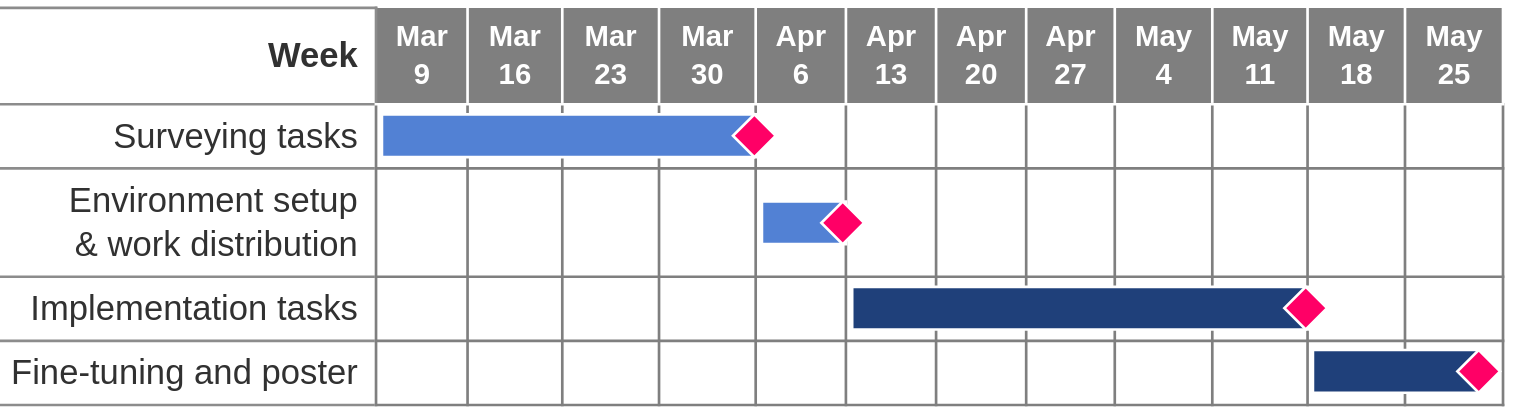
\includegraphics[width=\textwidth]{timeline.png}
	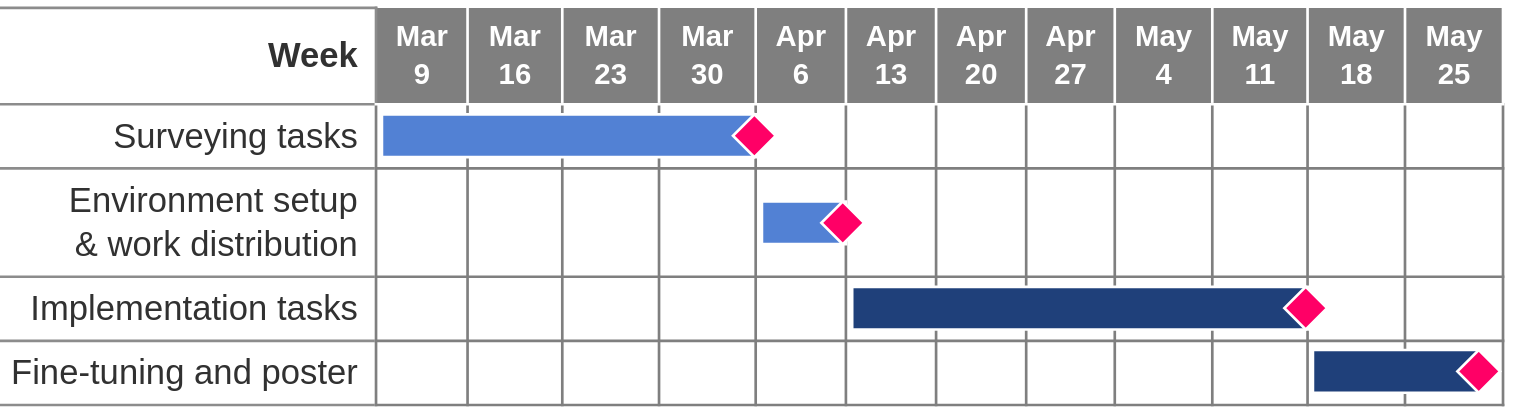
\includegraphics[height=3cm]{timeline.png}
\end{center}

\subsection{Challenges}
Many datasets for autonomous driving use different routes for their training set and their testing set because they are intended to be used for developing machine perception, e.g. detecting other cars, traffic signs, or pedestrians.
These datasets are not really useful to our project since localization using a map is only possible if the route of the evaluation data has been mapped before.
Thus, the initial challenge will be to find a dataset that sufficiently fulfills our requirements.
If we cannot find such a dataset we could generate our own.
For example, we could use image sequences from different cameras as a ``second run of the same route''.

Another challenge could be that the decisions we make as an initial step in the implementation turn out to be suboptimal for achieving satisfactory localization performance.
We might find that our chosen dataset does not include enough of the semantic features that we decided to use to localize accurately.
The conclusion would be that our semantic features are not prevalent enough on roads since the dataset should represent a real-world scenario. Hence, we should use a different set of features.
We will try to continuously reevaluate our decisions during the implementation phase.

Lastly, implementing the map computation, querying and position estimate could require a major time investment if we cannot find suitable existing implementations.

\section{Outcomes and Demonstration}
% Give detailed information on the expected outcome of your project and the experiments you plan to test your implementation. If applicable, describe the online or offline demo you plan to present at the end of the semester.

Of course, we want our localization to be as accurate as possible.
Generally, we want to achieve a level of accuracy that makes our approach usable for real-world scenarios.
However, we do not want to commit to specific numbers, which is why this statement is intentionally vague.

As an offline demo, we would like to present a video of semantic features being recognized and labeled from the car's point of view while simultaneously showing the current location estimate on the map.
If we manage to integrate our localization with a visual odometry pipeline we would like to show a comparison between localization with and without drift correction.

As an online demo we might set up an interactive environment for the audience to place objects (e.g. small road signs) in front of the camera under different lighting conditions to test the robustness of our system.
This part of our demo will mainly focus on feature detection.


{
	\small
\bibliographystyle{plain}
\bibliography{refs}
}

\end{document}
